% !TeX program = xelatex
\documentclass[UTF8,12pt,a4paper]{ctexart}
\usepackage{amsmath,amssymb}
\usepackage{geometry}
\usepackage{tikz} % 引入绘图包以生成几何图形
\geometry{margin=2cm}

% ===== 水印：贺昱琪学习资料 =====
\usepackage{xcolor}
\usepackage{eso-pic}
\usepackage{graphicx}

\newcommand{\WMText}{贺昱琪学习资料}
\newcommand{\WMScale}{2.28}
\newcommand{\WMAngle}{45}
\colorlet{WMColor}{black!8}

\AddToShipoutPictureBG{%
  \AtPageLowerLeft{%
    \put(\LenToUnit{0.66\paperwidth},\LenToUnit{0.70\paperheight}){%
      \rotatebox{\WMAngle}{\scalebox{\WMScale}{\textcolor{WMColor}{\WMText}}}%
    }%
    \put(\LenToUnit{0.33\paperwidth},\LenToUnit{0.50\paperheight}){%
      \rotatebox{\WMAngle}{\scalebox{\WMScale}{\textcolor{WMColor}{\WMText}}}%
    }%
    \put(\LenToUnit{0.66\paperwidth},\LenToUnit{0.30\paperheight}){%
      \rotatebox{\WMAngle}{\scalebox{\WMScale}{\textcolor{WMColor}{\WMText}}}%
    }%
  }%
}

% ===== 5题铺满一页布局 =====
\usepackage{enumitem}
\newcommand{\BottomWriteSpace}{1.5cm}

\newenvironment{OnePageFiveFill}{
  \small
  \vspace*{0pt}
  \begin{enumerate}[leftmargin=*, itemsep=0pt, topsep=0pt, parsep=0pt, partopsep=0pt]
  \setlength{\parskip}{0pt}
}{
  \end{enumerate}
  \vspace*{\BottomWriteSpace}
  \normalsize
  \newpage
}

\newcommand{\Q}[1]{\item #1\par\vfill}
\newcommand{\Qlast}[1]{\item #1\par}

\begin{document}

% =========================================================
% 6.1
% =========================================================
\section*{6月1日作业（5道题当晚22:00前打卡）}
\begin{OnePageFiveFill}

\Q{计算：$\displaystyle \frac{10 + \dfrac{1}{9}}{9 + \dfrac{1}{10}} - \frac{8 + \dfrac{1}{9}}{9 + \dfrac{1}{8}}$}

\Q{解方程组：$\begin{cases} 2x + y = 13 \\ \dfrac{x - 2}{3} = \dfrac{y - 1}{2} \end{cases}$}

\Q{
\begin{minipage}[c]{0.72\textwidth}
（三角形面积）如图所示，三角形 $ABC$ 的面积是 180 平方厘米，且三角形 $BDE$、三角形 $DEC$ 和三角形 $ACE$ 的面积都相等，求三角形 $ADE$ 的面积（涂色部分）。
\end{minipage}
\hfill
\begin{minipage}[c]{0.25\textwidth}
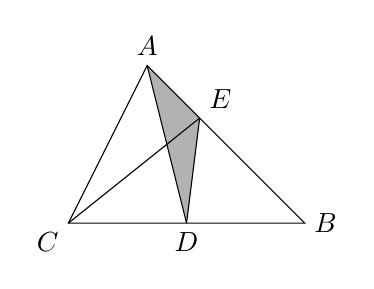
\begin{tikzpicture}[scale=0.5]
\coordinate (C) at (0,0); \coordinate (B) at (6,0); \coordinate (D) at (3,0);
\coordinate (A) at (2,4); \coordinate (E) at (3.333, 2.667);
\fill[black!30] (A) -- (D) -- (E) -- cycle;
\draw (A) -- (B) -- (C) -- cycle; \draw (A) -- (D); \draw (C) -- (E); \draw (D) -- (E);
\node[above] at (A) {$A$}; \node[right] at (B) {$B$}; \node[below left] at (C) {$C$};
\node[below] at (D) {$D$}; \node[above right] at (E) {$E$};
\end{tikzpicture}
\end{minipage}
}

\Q{（分数的应用）一辆汽车从甲地开往乙地。如果减速 $\dfrac{1}{10}$，则要比原定时间迟到 1 小时；如果以原速行驶 180 千米，再提速 $\dfrac{1}{5}$，则可比原定时间早到 1 小时。甲、乙两地的距离是多少千米？}

\Qlast{
\begin{minipage}[c]{0.75\textwidth}
（圆柱的体积）如图，一个盛有水的圆柱形玻璃容器的内底面半径为 10 cm，原容器内水的高度为 24 cm，把一根半径为 2 cm 的玻璃棒垂直插入水中后（触底），问容器内的水将升高多少厘米？
\end{minipage}
\hfill
\begin{minipage}[c]{0.22\textwidth}
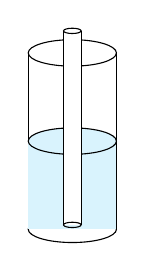
\begin{tikzpicture}[scale=0.28]
\draw (0,4) ellipse (2cm and 0.6cm); \draw (0,-4) ellipse (2cm and 0.6cm);
\draw (-2,-4) -- (-2,4); \draw (2,-4) -- (2,4);
\fill[cyan!15] (0,0) ellipse (2cm and 0.6cm); \fill[cyan!15] (-2,-4) rectangle (2,0);
\draw (0,0) ellipse (2cm and 0.6cm);
\fill[white] (-0.4,-3.8) rectangle (0.4, 5);
\draw (-0.4,-3.8) -- (-0.4, 5); \draw (0.4,-3.8) -- (0.4, 5);
\draw (0,5) ellipse (0.4cm and 0.12cm); \draw (0,-3.8) ellipse (0.4cm and 0.12cm);
\end{tikzpicture}
\end{minipage}
}

\end{OnePageFiveFill}

% =========================================================
% 6.2
% =========================================================
\section*{6月2日作业（5道题当晚22:00前打卡）}
\begin{OnePageFiveFill}

\Q{计算：$\displaystyle \frac{20 + \dfrac{1}{19}}{19 + \dfrac{1}{20}} - \frac{18 + \dfrac{1}{19}}{19 + \dfrac{1}{18}}$}

\Q{解方程组：$\begin{cases} 3x + 2y = 22 \\ \dfrac{x - 1}{3} = \dfrac{y - 3}{2} \end{cases}$}

\Q{
\begin{minipage}[c]{0.72\textwidth}
（三角形面积）如图所示，三角形 $ABC$ 的面积是 240 平方厘米，且三角形 $BDE$、三角形 $DEC$ 和三角形 $ACE$ 的面积都相等，求三角形 $ADE$ 的面积（涂色部分）。
\end{minipage}
\hfill
\begin{minipage}[c]{0.25\textwidth}
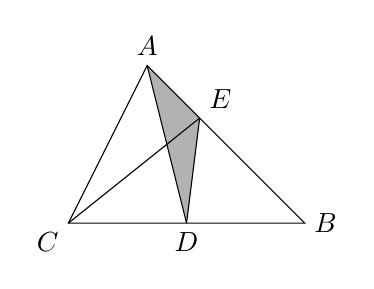
\begin{tikzpicture}[scale=0.5]
\coordinate (C) at (0,0); \coordinate (B) at (6,0); \coordinate (D) at (3,0);
\coordinate (A) at (2,4); \coordinate (E) at (3.333, 2.667);
\fill[black!30] (A) -- (D) -- (E) -- cycle;
\draw (A) -- (B) -- (C) -- cycle; \draw (A) -- (D); \draw (C) -- (E); \draw (D) -- (E);
\node[above] at (A) {$A$}; \node[right] at (B) {$B$}; \node[below left] at (C) {$C$};
\node[below] at (D) {$D$}; \node[above right] at (E) {$E$};
\end{tikzpicture}
\end{minipage}
}

\Q{（分数的应用）一辆汽车从甲地开往乙地。如果减速 $\dfrac{1}{5}$，则要比原定时间迟到 1 小时；如果以原速行驶 120 千米，再提速 $\dfrac{1}{3}$，则可比原定时间早到 0.5 小时。甲、乙两地的距离是多少千米？}

\Qlast{
\begin{minipage}[c]{0.75\textwidth}
（圆柱的体积）如图，一个盛有水的圆柱形玻璃容器的内底面半径为 6 cm，原容器内水的高度为 16 cm，把一根半径为 2 cm 的玻璃棒垂直插入水中后（触底），问容器内的水将升高多少厘米？
\end{minipage}
\hfill
\begin{minipage}[c]{0.22\textwidth}
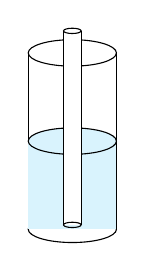
\begin{tikzpicture}[scale=0.28]
\draw (0,4) ellipse (2cm and 0.6cm); \draw (0,-4) ellipse (2cm and 0.6cm);
\draw (-2,-4) -- (-2,4); \draw (2,-4) -- (2,4);
\fill[cyan!15] (0,0) ellipse (2cm and 0.6cm); \fill[cyan!15] (-2,-4) rectangle (2,0);
\draw (0,0) ellipse (2cm and 0.6cm);
\fill[white] (-0.4,-3.8) rectangle (0.4, 5);
\draw (-0.4,-3.8) -- (-0.4, 5); \draw (0.4,-3.8) -- (0.4, 5);
\draw (0,5) ellipse (0.4cm and 0.12cm); \draw (0,-3.8) ellipse (0.4cm and 0.12cm);
\end{tikzpicture}
\end{minipage}
}

\end{OnePageFiveFill}

% =========================================================
% 6.3
% =========================================================
\section*{6月3日作业（5道题当晚22:00前打卡）}
\begin{OnePageFiveFill}

\Q{计算：$\displaystyle \frac{30 + \dfrac{1}{29}}{29 + \dfrac{1}{30}} - \frac{28 + \dfrac{1}{29}}{29 + \dfrac{1}{28}}$}

\Q{解方程组：$\begin{cases} x - y = 3 \\ \dfrac{x - 1}{2} = \dfrac{y + 5}{3} \end{cases}$}

\Q{
\begin{minipage}[c]{0.72\textwidth}
（三角形面积）如图所示，三角形 $ABC$ 的面积是 360 平方厘米，且三角形 $BDE$、三角形 $DEC$ 和三角形 $ACE$ 的面积都相等，求三角形 $ADE$ 的面积（涂色部分）。
\end{minipage}
\hfill
\begin{minipage}[c]{0.25\textwidth}
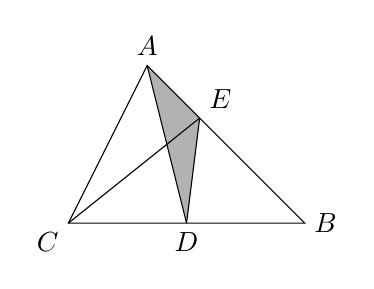
\begin{tikzpicture}[scale=0.5]
\coordinate (C) at (0,0); \coordinate (B) at (6,0); \coordinate (D) at (3,0);
\coordinate (A) at (2,4); \coordinate (E) at (3.333, 2.667);
\fill[black!30] (A) -- (D) -- (E) -- cycle;
\draw (A) -- (B) -- (C) -- cycle; \draw (A) -- (D); \draw (C) -- (E); \draw (D) -- (E);
\node[above] at (A) {$A$}; \node[right] at (B) {$B$}; \node[below left] at (C) {$C$};
\node[below] at (D) {$D$}; \node[above right] at (E) {$E$};
\end{tikzpicture}
\end{minipage}
}

\Q{（分数的应用）一辆汽车从甲地开往乙地。如果减速 $\dfrac{1}{6}$，则要比原定时间迟到 1 小时；如果以原速行驶 200 千米，再提速 $\dfrac{1}{4}$，则可比原定时间早到 0.6 小时。甲、乙两地的距离是多少千米？}

\Qlast{
\begin{minipage}[c]{0.75\textwidth}
（圆柱的体积）如图，一个盛有水的圆柱形玻璃容器的内底面半径为 8 cm，原容器内水的高度为 12 cm，把一根半径为 4 cm 的玻璃棒垂直插入水中后（触底），问容器内的水将升高多少厘米？
\end{minipage}
\hfill
\begin{minipage}[c]{0.22\textwidth}
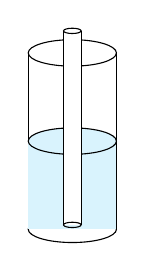
\begin{tikzpicture}[scale=0.28]
\draw (0,4) ellipse (2cm and 0.6cm); \draw (0,-4) ellipse (2cm and 0.6cm);
\draw (-2,-4) -- (-2,4); \draw (2,-4) -- (2,4);
\fill[cyan!15] (0,0) ellipse (2cm and 0.6cm); \fill[cyan!15] (-2,-4) rectangle (2,0);
\draw (0,0) ellipse (2cm and 0.6cm);
\fill[white] (-0.4,-3.8) rectangle (0.4, 5);
\draw (-0.4,-3.8) -- (-0.4, 5); \draw (0.4,-3.8) -- (0.4, 5);
\draw (0,5) ellipse (0.4cm and 0.12cm); \draw (0,-3.8) ellipse (0.4cm and 0.12cm);
\end{tikzpicture}
\end{minipage}
}

\end{OnePageFiveFill}

% =========================================================
% 6.4
% =========================================================
\section*{6月4日作业（5道题当晚22:00前打卡）}
\begin{OnePageFiveFill}

\Q{计算：$\displaystyle \frac{40 + \dfrac{1}{39}}{39 + \dfrac{1}{40}} - \frac{38 + \dfrac{1}{39}}{39 + \dfrac{1}{38}}$}

\Q{解方程组：$\begin{cases} x + 4y = 14 \\ \dfrac{x}{3} = \dfrac{y + 2}{2} \end{cases}$}

\Q{
\begin{minipage}[c]{0.72\textwidth}
（三角形面积）如图所示，三角形 $ABC$ 的面积是 420 平方厘米，且三角形 $BDE$、三角形 $DEC$ 和三角形 $ACE$ 的面积都相等，求三角形 $ADE$ 的面积（涂色部分）。
\end{minipage}
\hfill
\begin{minipage}[c]{0.25\textwidth}
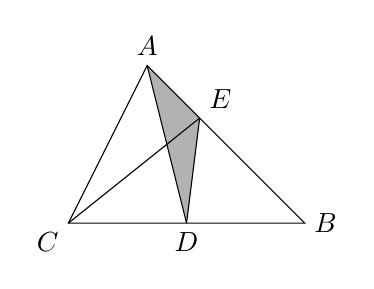
\begin{tikzpicture}[scale=0.5]
\coordinate (C) at (0,0); \coordinate (B) at (6,0); \coordinate (D) at (3,0);
\coordinate (A) at (2,4); \coordinate (E) at (3.333, 2.667);
\fill[black!30] (A) -- (D) -- (E) -- cycle;
\draw (A) -- (B) -- (C) -- cycle; \draw (A) -- (D); \draw (C) -- (E); \draw (D) -- (E);
\node[above] at (A) {$A$}; \node[right] at (B) {$B$}; \node[below left] at (C) {$C$};
\node[below] at (D) {$D$}; \node[above right] at (E) {$E$};
\end{tikzpicture}
\end{minipage}
}

\Q{（分数的应用）一辆汽车从甲地开往乙地。如果减速 $\dfrac{1}{4}$，则要比原定时间迟到 2 小时；如果以原速行驶 180 千米，再提速 $\dfrac{1}{2}$，则可比原定时间早到 1 小时。甲、乙两地的距离是多少千米？}

\Qlast{
\begin{minipage}[c]{0.75\textwidth}
（圆柱的体积）如图，一个盛有水的圆柱形玻璃容器的内底面半径为 9 cm，原容器内水的高度为 16 cm，把一根半径为 3 cm 的玻璃棒垂直插入水中后（触底），问容器内的水将升高多少厘米？
\end{minipage}
\hfill
\begin{minipage}[c]{0.22\textwidth}
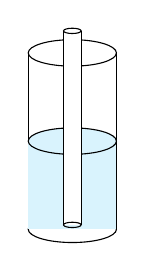
\begin{tikzpicture}[scale=0.28]
\draw (0,4) ellipse (2cm and 0.6cm); \draw (0,-4) ellipse (2cm and 0.6cm);
\draw (-2,-4) -- (-2,4); \draw (2,-4) -- (2,4);
\fill[cyan!15] (0,0) ellipse (2cm and 0.6cm); \fill[cyan!15] (-2,-4) rectangle (2,0);
\draw (0,0) ellipse (2cm and 0.6cm);
\fill[white] (-0.4,-3.8) rectangle (0.4, 5);
\draw (-0.4,-3.8) -- (-0.4, 5); \draw (0.4,-3.8) -- (0.4, 5);
\draw (0,5) ellipse (0.4cm and 0.12cm); \draw (0,-3.8) ellipse (0.4cm and 0.12cm);
\end{tikzpicture}
\end{minipage}
}

\end{OnePageFiveFill}

% =========================================================
% 6.5
% =========================================================
\section*{6月5日作业（5道题当晚22:00前打卡）}
\begin{OnePageFiveFill}

\Q{计算：$\displaystyle \frac{50 + \dfrac{1}{49}}{49 + \dfrac{1}{50}} - \frac{48 + \dfrac{1}{49}}{49 + \dfrac{1}{48}}$}

\Q{解方程组：$\begin{cases} 5x - y = 2 \\ \dfrac{x + 4}{3} = \dfrac{y}{4} \end{cases}$}

\Q{
\begin{minipage}[c]{0.72\textwidth}
（三角形面积）如图所示，三角形 $ABC$ 的面积是 480 平方厘米，且三角形 $BDE$、三角形 $DEC$ 和三角形 $ACE$ 的面积都相等，求三角形 $ADE$ 的面积（涂色部分）。
\end{minipage}
\hfill
\begin{minipage}[c]{0.25\textwidth}
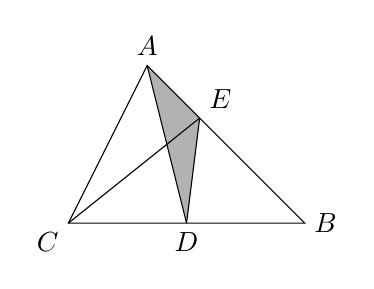
\begin{tikzpicture}[scale=0.5]
\coordinate (C) at (0,0); \coordinate (B) at (6,0); \coordinate (D) at (3,0);
\coordinate (A) at (2,4); \coordinate (E) at (3.333, 2.667);
\fill[black!30] (A) -- (D) -- (E) -- cycle;
\draw (A) -- (B) -- (C) -- cycle; \draw (A) -- (D); \draw (C) -- (E); \draw (D) -- (E);
\node[above] at (A) {$A$}; \node[right] at (B) {$B$}; \node[below left] at (C) {$C$};
\node[below] at (D) {$D$}; \node[above right] at (E) {$E$};
\end{tikzpicture}
\end{minipage}
}

\Q{（分数的应用）一辆汽车从甲地开往乙地。如果减速 $\dfrac{1}{8}$，则要比原定时间迟到 1 小时；如果以原速行驶 140 千米，再提速 $\dfrac{1}{6}$，则可比原定时间早到 0.5 小时。甲、乙两地的距离是多少千米？}

\Qlast{
\begin{minipage}[c]{0.75\textwidth}
（圆柱的体积）如图，一个盛有水的圆柱形玻璃容器的内底面半径为 12 cm，原容器内水的高度为 20 cm，把一根半径为 4 cm 的玻璃棒垂直插入水中后（触底），问容器内的水将升高多少厘米？
\end{minipage}
\hfill
\begin{minipage}[c]{0.22\textwidth}
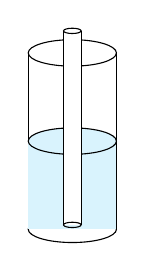
\begin{tikzpicture}[scale=0.28]
\draw (0,4) ellipse (2cm and 0.6cm); \draw (0,-4) ellipse (2cm and 0.6cm);
\draw (-2,-4) -- (-2,4); \draw (2,-4) -- (2,4);
\fill[cyan!15] (0,0) ellipse (2cm and 0.6cm); \fill[cyan!15] (-2,-4) rectangle (2,0);
\draw (0,0) ellipse (2cm and 0.6cm);
\fill[white] (-0.4,-3.8) rectangle (0.4, 5);
\draw (-0.4,-3.8) -- (-0.4, 5); \draw (0.4,-3.8) -- (0.4, 5);
\draw (0,5) ellipse (0.4cm and 0.12cm); \draw (0,-3.8) ellipse (0.4cm and 0.12cm);
\end{tikzpicture}
\end{minipage}
}

\end{OnePageFiveFill}

\end{document}